\chapter{BLAS}
Die Abkürzung BLAS steht für Basic Linear Algebra Subprograms. 
BLAS-Bibliotheken enthalten elementare Operationen der linearen Algebra.


\section{Datenstruktur für Matrizen}
Vollbesetzte Matrizen werden bei BLAS entweder zeilen- oder spaltenweise abgespeichert. Das bedeutet, dass entweder die Zeilen- oder die Spalten der Matrix hintereinander im Speicher stehen.  

\begin{align*}
	A=
	\left(\begin{array}{ccc}
	a_{1,1} & a_{1,2} & a_{1,3} \\ 
	a_{2,1} & a_{2,2} & a_{2,3} \\ 
	a_{3,1} & a_{3,2} & a_{3,3} 
	\end{array} \right) \in \mathbb{R}^{3 \times 3}
\end{align*}
Matrix $A$ Zeilenweise gespeichert\\
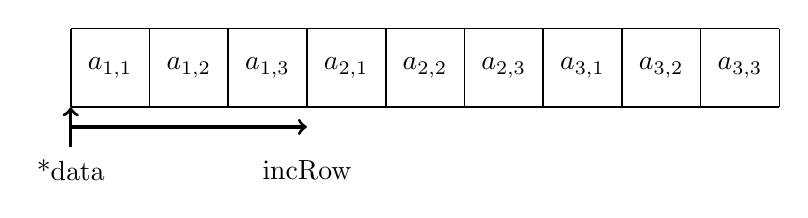
\begin{tikzpicture}
	\draw[semithick] (0,0) -- (9,0);
	\draw[semithick] (0,1) -- (9,1);
	\draw[semithick] (0,0) -- (0,1);
	\draw[semithick] (1,0) -- (1,1);
	\draw[semithick] (2,0) -- (2,1);
	\draw[semithick] (3,0) -- (3,1);
	\draw[semithick] (4,0) -- (4,1);
	\draw[semithick] (5,0) -- (5,1);
	\draw[semithick] (6,0) -- (6,1);
	\draw[semithick] (7,0) -- (7,1);
	\draw[semithick] (8,0) -- (8,1);
	\draw[semithick] (9,0) -- (9,1);
	
	\draw (0.5,0.5) node {$a_{1,1}$};
	\draw (1.5,0.5) node {$a_{1,2}$};
	\draw (2.5,0.5) node {$a_{1,3}$};
	\draw (3.5,0.5) node {$a_{2,1}$};
	\draw (4.5,0.5) node {$a_{2,2}$};
	\draw (5.5,0.5) node {$a_{2,3}$};
	\draw (6.5,0.5) node {$a_{3,1}$};
	\draw (7.5,0.5) node {$a_{3,2}$};
	\draw (8.5,0.5) node {$a_{3,3}$};
	
	\draw[->,line width=0.4mm] (0,-.5) -- (0,0);
	\draw (0,-0.8) node {*data};
	\draw[->,line width=0.4mm] (0,-.25) -- (3,-.25);
	\draw (3,-0.8) node {incRow};
\end{tikzpicture}\\
Matrix $A$ Spaltenweise gespeichert\\
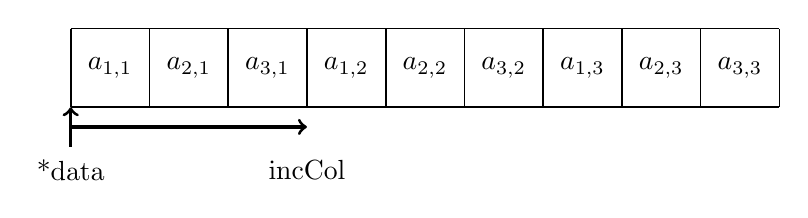
\begin{tikzpicture}
\draw[semithick] (0,0) -- (9,0);
\draw[semithick] (0,1) -- (9,1);
\draw[semithick] (0,0) -- (0,1);
\draw[semithick] (1,0) -- (1,1);
\draw[semithick] (2,0) -- (2,1);
\draw[semithick] (3,0) -- (3,1);
\draw[semithick] (4,0) -- (4,1);
\draw[semithick] (5,0) -- (5,1);
\draw[semithick] (6,0) -- (6,1);
\draw[semithick] (7,0) -- (7,1);
\draw[semithick] (8,0) -- (8,1);
\draw[semithick] (9,0) -- (9,1);

\draw (0.5,0.5) node {$a_{1,1}$};
\draw (1.5,0.5) node {$a_{2,1}$};
\draw (2.5,0.5) node {$a_{3,1}$};
\draw (3.5,0.5) node {$a_{1,2}$};
\draw (4.5,0.5) node {$a_{2,2}$};
\draw (5.5,0.5) node {$a_{3,2}$};
\draw (6.5,0.5) node {$a_{1,3}$};
\draw (7.5,0.5) node {$a_{2,3}$};
\draw (8.5,0.5) node {$a_{3,3}$};
	
\draw[->,line width=0.4mm] (0,-.5) -- (0,0);
\draw (0,-0.8) node {*data};
\draw[->,line width=0.4mm] (0,-.25) -- (3,-.25);
\draw (3,-0.8) node {incCol};
\end{tikzpicture}\\


Eine Datenstruktur benötigt folgende Elemente:
\begin{itemize}
	\item einen Zeiger auf eine Speicherfläche
	\item Information, ob die Matrix zeilen- oder spaltenweise gespeichert ist 
	\item die Dimension der Matrix.
\end{itemize}


Eine derartige Datenstruktur könnte in C/C++ so aussehen.
\begin{lstlisting}
struct Matrix {
  double * data;
  std::ptrdiff_t incRow, incCol;
  std::size_t numRows, numCols;
}
\end{lstlisting}

Diese Datenstruktur ist für Matrixeinträge vom Type double.
Die Variablen für die Speicherverwaltung(Zeile 3) sind vom Typ \textit{ptrdiff\_t} und die Variablen für die Dimensions Informationen sind vom Typ \textit{size\_t}.
\textit{ptrdiff\_t} und \textit{size\_t} sind Datentypen für Ganzzahlen. Der Unterschied zwischen den Datentypen ist \textit{size\_t} kann nur Werte Darstellen die $\geq$ 0 sind, \textit{ptrdiff\_t} dann auch negative Werte darstellen.
Die das \textit{incRow} und \textit{incCol} aus negative Werte haben könne ist Sinnvoll, wenn man zugriff auf Einen Matrix Block haben will in anderer Reihenfolge. \cite{blast}

Für Intel-MKL-Routinen müssen die Matrizen zeilenweise gespeichert sein.
Das bedeutet \textit{incCol} ist gleich 1.

\subsubsection{Beispiel}
Angenommen, es wurde genügend Speicher für eine Matrix $A$ belegt und die Werte 1 bis 25 liegen hintereinander im Speicher.
Dann lässt sich die Matrix
\begin{align*}
	A = \begin{pmatrix}
	 1 &  2 &  3 &  4 &  5 \\
	 6 &  7 &  8 &  9 & 10 \\
	11 & 12 & 13 & 14 & 15 \\
	16 & 17 & 18 & 19 & 20 \\
	21 & 22 & 23 & 24 & 25 
	\end{pmatrix}
\end{align*}
durch die folgende Datenstruktur repräsentieren.
\begin{lstlisting}
struct Matrix A;
A.data = /*pointer to data*/;
A.numRows = 5; 
A.numCols = 5;
A.incRow = A.numCols;
A.incCol = 1;
\end{lstlisting}

Die Matrix $B$ soll den Matrixblock aus $A$ darstellen, welcher in der zweiten Zeile und dritte Spalte beginnt. Zusätzlich soll der Block transponiert betrachtet werden. Die Matrix
\begin{align*}
B = \begin{pmatrix}
8 &  13 &  18 & 23 \\
9 &  14 &  19 & 24 \\
10 &  15 &  20 & 25 
\end{pmatrix}
\end{align*}
lässt sich mit folgender Datenstruktur repräsentieren.
\begin{lstlisting}
struct Matrix B;
B.data = &A.data[ 1*A.incRow + 2*A.incCol ];
B.numRows = 3; 
B.numCols = 4;
B.incRow = A.incCol;
B.incCol = A.incRow;
\end{lstlisting}

In Zeile 2 wird der Daten-Zeiger auf das Element der zweiten Zeile und dritten Spalte gesetzt.
Um die Matrix zu transponieren, werden die Inkremente vertauscht. Dies geschieht in den Zeilen 5 und 6.  
In den Zeilen 3 und 4 wird die Matrix Dimensionen richtig gesetzt.

Die Matrix $C$ soll ein Beispiel für negative Inkremente sein. Sie nutzt den selben Datenspeicher wie die Matrizen $A$ und $B$, in dem die Werte 1 bis 25 hintereinander im Speicher liegen.
Die Matrix 
\begin{align*}
C = \begin{pmatrix}
25 &  20 &  15 & 10 \\
24 &  19 &  14 & 9 \\
23 &  18 &  13 & 8 
\end{pmatrix}
\end{align*}
lässt sich mit folgender Datenstruktur repräsentieren.
\begin{lstlisting}
struct Matrix C;
C.data = &B.data[ 2*B.incRow + 3*B.incCol ];
C.numRows = B.numRows; 
C.numCols = B.numCols;
C.incRow = -B.incRow;
C.incCol = -B.incCol;
\end{lstlisting}
Der data-Pointer wurde auf das letzte Element der Matrix $B$ gesetzt. Die Inkremente werden negativ von der Matrix $B$ übernommen.

Matrizen wie $B$ und $C$, die den selben Datenspeicher wie $A$ nutzen, werden als Matrixview bezeichnet. \cite{blast}


\newpage
\section{Einige BLAS-Routinen}
Im Folgenden werden einige BLAS-Routinen beschrieben, die bei der QR-Zerlegung benutzt werden.
BLAS-Routinen werden nach folgendem Schema benannt:
Der erste Buchstabe im Namen gibt an, für welchen Datentyp die Funktion implementiert wurde. Der Rest beschreibt die Funktion.\\
Beispiel \glqq dgemm\grqq{}: Das \glqq d\grqq{} zeigt, dass die Funktion für Doubles gilt und  \glqq gemm\grqq{} steht für \glqq general matrix matrix\grqq{}. Die  Funktion berechnet also das Matrix-Matrix Produkt für Matrizen, deren Einträge Doubles sind.

\subsection{Matrix-Matrix Produkt (gemm)}
Die Funktion \glqq gemm\grqq{} berechnet das Matrix-Matrix Produkt.
Der Funktion werden die Matrizen $A$, $B$ und $C$ und die Skalare $\alpha$ und $\beta$ übergeben. Außerdem werden zwei Flags übergeben, ob die Matrizen $A$ und $B$ transponiert zu betrachten sind.\\
Die Funktion berechnet
\begin{align}
	C \leftarrow \beta  C + \alpha  A  B
\end{align}
Falls $\beta = 0$, wird die Matrix $C$ zuerst mit Nullen initialisiert. Falls $C$ Einträge hat, die NaN (\textit{Not a Number}) sind, werden diese mit Nullen überschrieben.

%%TODO
\cite{blast}
Blas tecnical forum netlib
%%http://www.netlib.org/blas/blast-forum/

\subsection{Matrix-Vektor Produkt (gemv)}
Die Funktion \glqq gemv\grqq{} berechnet das Matrix-Vektor Produkt.
Der Funktion werden die Matrix $A$, die Vektoren $x$ und $y$, und die Skalare $\alpha$ und $\beta$ übergeben. Außerdem wird ein Flag übergeben, das anzeigt, ob die Matrix $A$ transponiert werden soll.\\
Die Funktion berechnet
\begin{align}
y \leftarrow \beta  y + \alpha A x 
\end{align}
Falls $\beta = 0$, wird der Vektor $y$ zuerst mit Nullen initialisiert. Falls $y$ Einträge hat, die NaN (\textit{Not a Number}) sind, werden diese mit Nullen überschrieben.

\subsection{Rank1 update (ger)}
Die Funktion \glqq ger\grqq{}  berechnet ein dyadisches Produkt aus den Vektoren $x$ und $y$, skaliert die daraus resultierende Matrix mit $\alpha$ und addiert das Ergebnis auf $A$.\\
Der Funktion werden die Matrix $A$, die Vektoren $x$ und $y$ und das Skalar $\alpha$ übergeben.\\
Die Funktion berechnet
\begin{align}
A \leftarrow A + \alpha  x y^T
\end{align}

\subsection{Matrix-Matrix Produkt (trmm)} \label{fkt:trmm}
Die Funktion \glqq trmm\grqq{} berechnet das Matrix-Matrix-Produkt einer Dreiecksmatrix mit einer voll besetzten Matrix.
Der Funktion wird die Dreiecksmatrix $A$, die Matrix $B$ und das Skalar $\alpha$ übergeben. Außerdem werden Flags mit übergeben, die anzeigen, ob $A$ eine obere oder untere Dreiecksmatrix ist, ob $A$ eine strikte oder unipotente Dreiecksmatrix ist, ob $A$ von links oder rechts auf $B$ multipliziert werden soll und ob $A$ transponiert werden soll. Diese Eigenschaften werden unten in $op(\cdot)$ zusammengefasst. \\
Die Funktion berechnet
\begin{align}
B \leftarrow  \alpha \cdot op(A) \cdot B \qquad \text{oder} \qquad B \leftarrow  \alpha \cdot B \cdot op(A)
\end{align}
\subsection{Matrix-Vektor Produkt (trmv)} \label{fkt:trmv}
Die Funktion \glqq trmv\grqq{} berechnet das Matrix-Vektor-Produkt für Dreiecksmatrizen.
Die Funktion berechnet
\begin{align}
x \leftarrow \alpha  Ax %\qquad \text{or} \qquad x \leftarrow \alpha * A^T*x
\end{align}


Dreiecksmatrizen, die von den Funktionen \glqq trmm\grqq{} und \glqq trmv\grqq{} verarbeitet werden, sind quadratische Matrizen, von denen nur der obere oder der untere Dreiecksteil betrachtet wird.
Das heißt, die Matrix liegt als quadratische Matrix im Speicher. Die Funktion beachtet nur die Einträge über oder unter der Diagonalen.
Wird dem Algorithmus mit einem Flag angezeigt, dass 
er die Matrix als eine unipotente Dreiecksmatrix betrachten soll,
%es sich um eine eine unipotente Dreiecksmatrix handeln soll, 
dann werden die Diagonaleinträge im Speicher nicht beachtet, sondern vom Algorithmus als 1 angenommen. \cite{blast}


